\section{Validation and Results}
\label{sec:validation_results}

Validation proceeds from global surface statistics to localized curling-wave geometry and scattering, and finally to full-scene radar signatures and computational efficiency. Accordingly, the evaluation is organized into five levels: large-area slope statistics, local curling-wave geometry, local electromagnetic scattering, full-scene radar echoes, and computational scalability.






\subsection{Global Surface Statistical Validation}
\label{subsec:global_surface_validation}

This subsection examines whether the generated large-area surfaces retain physically plausible wind-dependent roughness before the localized curling operation is introduced. Three related questions are separated: whether the multiscale linear generator recovers the mean-square slope (MSS) implied by its input Elfouhaily spectrum, whether the MSS-constrained nonlinear surface remains consistent with observation-based low- and moderate-wind slope statistics, and whether its total MSS exhibits a plausible flattening trend under high sea states. The second comparison is a constraint-compliance test rather than a fully independent prediction test because the accepted implementation uses Cox--Munk, Hu/TGRS, and Gu\'erin data to construct the nonlinear MSS target; the subsequent geometry and electromagnetic tests therefore provide the independent evidence for the nonlinear structures.

Let $\widehat{\eta}(\boldsymbol{k})$ denote the Fourier coefficient of a synthesized surface, and let $k_a$ and $k_c$ be the along- and cross-wind wavenumber components defined in Section~II. The directional and total MSSs and the anisotropy factor are calculated directly from the resolved spectral coefficients as
\begin{equation}
\begin{aligned}
m_a&=\sum_{\boldsymbol{k}}k_a^2
\left|\widehat{\eta}(\boldsymbol{k})\right|^2,
&
m_c&=\sum_{\boldsymbol{k}}k_c^2
\left|\widehat{\eta}(\boldsymbol{k})\right|^2,
\\
m_t&=m_a+m_c,
&
\gamma&=\left(\frac{m_c}{m_a}\right)^{1/2}.
\end{aligned}
\label{eq:validation_mss_metrics}
\end{equation}

The primary grid uses $\Delta k=k_p/12$ and resolves nonlinear interactions up to $8k_p$. Independent octave tiles then represent the unresolved short-wave bands up to $k_{\max}=1000\pi~\mathrm{rad/m}$. Because the tiles occupy disjoint wavenumber bands, their slope variances are added to the primary-band moments. This multiscale construction includes the gravity--capillary contribution needed for comparison with optical-scale slope statistics without requiring one millimeter-spaced grid over the entire sea-surface domain.

For the low- and moderate-wind experiment, the Cox--Munk reference is evaluated after converting the simulated 10-m wind speed to the 12.5-m wind convention, $U_{12.5}=U_{10}/0.98$. Its directional components are~\cite{cox1954measurement}
\begin{equation}
\begin{aligned}
m_{a,\mathrm{CM}}&=3.16\times10^{-3}U_{12.5},\\
m_{c,\mathrm{CM}}&=3.00\times10^{-3}
+1.92\times10^{-3}U_{12.5}.
\end{aligned}
\label{eq:cox_munk_directional_mss}
\end{equation}

The comparison is made primarily against observation-derived sea-surface
slope statistics rather than against MSS values obtained from other
numerically simulated sea surfaces. Cox--Munk provides an empirical
wind-dependent slope relation derived from measured ocean-surface
sun-glitter statistics~\cite{cox1954measurement}. The direction-resolved
Gu\'erin values are retrieved from IASI observations over their available
wind interval~\cite{guerin2023seasurfaceslope}, while the Hu/TGRS relation
represents an observation-based wind-dependent MSS parameterization
summarized in the generalized sea-surface slope model~\cite{gao2024generalized}.
Accordingly, these curves are used as measured or empirically retrieved
statistical references, not as outputs of competing sea-surface simulation
algorithms.

For comparison, the ``Elfouhaily et al.--Unified spectrum'' curve is of a
different nature: it is obtained by numerically integrating the directional
Elfouhaily spectrum implemented in the present generator and therefore serves
as an internal spectral-consistency reference rather than an independent
measurement. The component-wise arithmetic mean of the available Cox--Munk,
Hu/TGRS, and Gu\'erin statistics is used only to construct the low- and
moderate-wind MSS constraint target and is denoted as the fusion constraint
below.


\begin{equation}
m_{q,\mathrm{des}}
=
m_{q,\mathrm{tar}}
\left(
\frac{m_{q,\mathrm{raw}}}
     {m_{q,\mathrm{tar}}}
\right)^{\rho},
\qquad q\in\{a,c\},
\label{eq:mss_log_domain_contraction}
\end{equation}
where $\rho=0.15$ retains part of the realization-to-realization deviation. The positive angular dressing in Section~II is then solved to realize $m_{a,\mathrm{des}}$ and $m_{c,\mathrm{des}}$ without changing Fourier phase. 
Thus, the two simulated groups evaluated here are the linear Elfouhaily
realization and the proposed MSS-constrained Modified-Lie realization.
Cox--Munk, Hu/TGRS, and Gu\'erin are not additional simulated groups; they
provide observation-derived statistical reference values against which the
simulated MSS is assessed.

Wind speed is varied from $1$ to $10~\mathrm{m/s}$ in $1~\mathrm{m/s}$ increments, with 20 paired realizations at every wind speed. At each condition, the median is used as the central estimate, while the Monte Carlo spread is retained in the statistical summaries. Agreement with a reference curve $r_i$ is summarized by
\begin{equation}
\operatorname{RMSE}
=
\left[
\frac{1}{N_U}
\sum_{i=1}^{N_U}
\left(
\widetilde{m}_{t,i}-r_i
\right)^2
\right]^{1/2},
\label{eq:mss_rmse}
\end{equation}
where $\widetilde{m}_{t,i}$ is the median total MSS at the $i$th wind speed.

Figure~\ref{fig:global_mss_low_wind} compares the total and directional MSSs over the low- and moderate-wind interval. Plotting $m_a$ and $m_c$ separately is useful because agreement in total MSS alone does not guarantee that the slope variance is distributed correctly between the along- and cross-wind directions.

\begin{figure}[!t]
    \centering
    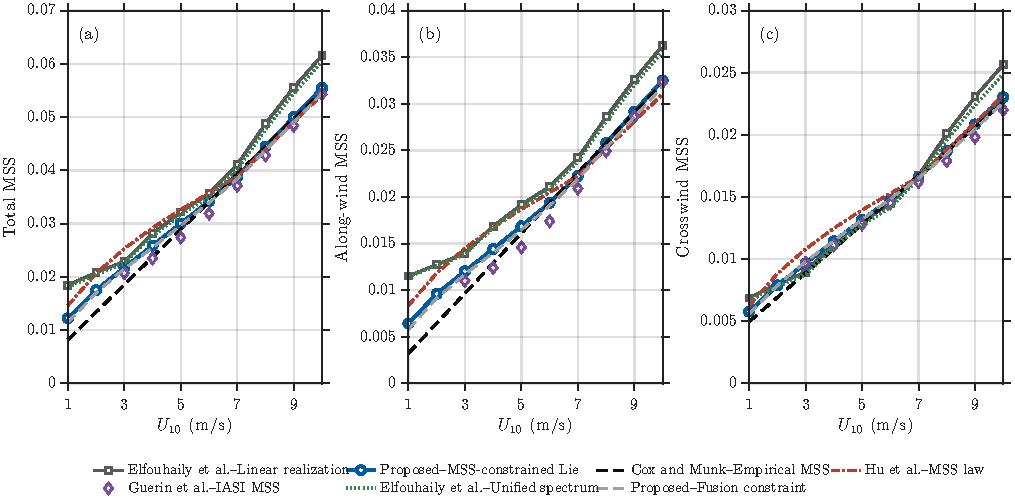
\includegraphics[width=\columnwidth]
    {plotcode/CoxMunk_IEEE_plotting_updated/output/Fig_low_moderate_mss_validation.pdf}
    \caption{Low- and moderate-wind MSS comparison for
    $U_{10}=1$--$10~\mathrm{m/s}$ using 20 paired realizations per wind
    speed. (a) Total MSS. (b) Along-wind MSS. (c) Crosswind MSS.
    The two simulated groups are compared with observation-derived
    Cox--Munk, Hu et al., and Gu\'erin slope statistics. The integrated
    Elfouhaily curve is a spectrum-based internal reference rather than a
    measurement, while the fusion curve denotes the statistical constraint
    used by the proposed model and is not an independent observation.}
    \label{fig:global_mss_low_wind}
\end{figure}

As shown in Fig.~\ref{fig:global_mss_low_wind}(a), the linear realizations closely reproduce the numerical integral of the implemented Elfouhaily spectrum, with an RMSE of $7.53\times10^{-4}$. This confirms the self-consistency of the spectral sampling, octave-band accumulation, and MSS calculation. Their total MSS nevertheless increasingly exceeds the Cox--Munk and Gu\'erin references toward the upper end of the interval: the median rises from 0.01846 at $1~\mathrm{m/s}$ to 0.06156 at $10~\mathrm{m/s}$, whereas the corresponding Cox--Munk values are 0.00818 and 0.05484. After directional moment contraction, the nonlinear medians become 0.01221 and 0.05547, respectively, and remain monotonic over the complete wind interval. Figures~\ref{fig:global_mss_low_wind}(b) and \ref{fig:global_mss_low_wind}(c) further show that the correction acts consistently on the along- and cross-wind slope components rather than matching the total MSS through compensation between the two directions.

The quantitative errors exhibit the same behavior. Relative to the linear baseline, the constrained nonlinear group reduces the total-MSS RMSE from 0.00560 to 0.00223 against Cox--Munk, from 0.00523 to 0.00188 against the available Gu\'erin values, and from 0.00383 to 0.00227 against the Hu/TGRS law. Its RMSE relative to the fusion target is $6.28\times10^{-4}$, compared with 0.00456 for the linear group. The mean absolute anisotropy error relative to the TGRS value decreases from 0.04699 to 0.02678. The constrained $\gamma$ changes from 0.948 at $1~\mathrm{m/s}$ to 0.841 at $10~\mathrm{m/s}$; its elevated low-wind value follows partly from the constant crosswind term in the Cox--Munk law and should therefore be interpreted as a property of the adopted directional constraint rather than as an independently predicted nonlinear-wave effect.

The high-sea-state experiment tests a different statistical behavior.
No competing numerically simulated sea surface is used as the high-wind
reference. Instead, the comparison is made with the observation-based
Hu/TGRS MSS parameterization. The Cox--Munk relation is retained in the
figure only to illustrate the consequence of linearly extrapolating its
classical empirical trend beyond the moderate-wind regime. For $U_{10}\geq13.3~\mathrm{m/s}$, the accepted implementation adopts the logarithmic Hu/TGRS branch
\begin{equation}
m_{t,\mathrm{Hu}}
=
0.138\log_{10}U_{10}-0.084,
\label{eq:hu_high_wind_mss}
\end{equation}
while the lower part of this experiment uses its adjacent linear branch. The test covers $U_{10}=10:2:40~\mathrm{m/s}$ with 20 paired realizations per condition and retains $\rho=0.05$. In addition to the linear and constrained groups, the raw Modified-Lie result is reported to expose the effect of the statistical constraint. High-wind behavior is measured by the RMSE to the Hu/TGRS target, the ratio between the mean tail slope above $24~\mathrm{m/s}$ and the early slope below $16~\mathrm{m/s}$, and the fraction of successive slope intervals that are concave. Figure~\ref{fig:global_mss_high_wind} shows both the resulting total MSS and its finite-difference growth rate.

\begin{figure}[!t]
    \centering
    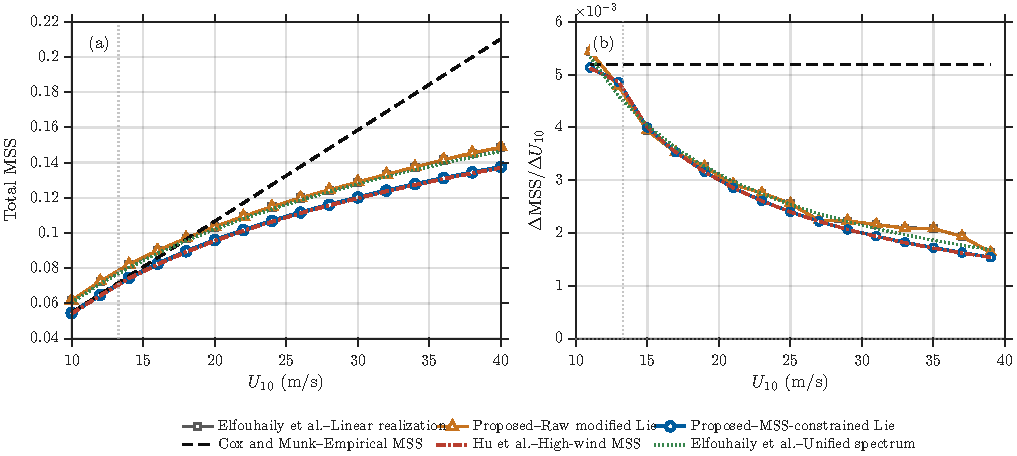
\includegraphics[width=\columnwidth]
    {plotcode/CoxMunk_IEEE_plotting_updated/output_high_sea_state/Fig_high_sea_state_mss_validation.pdf}
    \caption{High-sea-state MSS behavior for
    $U_{10}=10$--$40~\mathrm{m/s}$ using 20 paired realizations per wind
    speed. (a) Median total MSS of the linear Elfouhaily, raw Modified-Lie,
    and proposed MSS-constrained Lie realizations. The Hu et al. curve is
    used as the observation-based high-wind MSS reference, the Cox--Munk
    curve is shown only as a linear empirical extrapolation for comparison,
    and the integrated Elfouhaily curve is a spectrum-based model reference.
    The vertical marker at $U_{10}=13.3~\mathrm{m/s}$ denotes the transition
    to the logarithmic Hu high-wind branch. (b) Finite-difference MSS growth
    rate $\Delta\mathrm{MSS}/\Delta U_{10}$, illustrating the progressive
    reduction in wind-speed sensitivity at high sea states.}
    \label{fig:global_mss_high_wind}
\end{figure}

As shown in Fig.~\ref{fig:global_mss_high_wind}(a), the raw Modified-Lie correction alone changes the total MSS only slightly and yields an RMSE of 0.00911, compared with 0.00900 for the linear realizations and 0.00757 for the continuous Elfouhaily integral. The constrained group reduces this value to $3.96\times10^{-4}$. Its median total MSS increases from 0.05455 at $10~\mathrm{m/s}$ to 0.13754 at $40~\mathrm{m/s}$ and remains strictly monotonic. More importantly, Fig.~\ref{fig:global_mss_high_wind}(b) shows that its finite-difference growth rate decreases progressively with increasing wind speed rather than remaining approximately constant as in a linear extrapolation. The resulting tail-to-early slope ratio is 0.411, and all evaluated slope intervals satisfy the adopted concavity criterion.

Together, the two experiments show that the multiscale generator reproduces its prescribed spectral slope energy and that the accepted statistical constraint prevents the nonlinear transform from producing unbounded or incorrectly distributed MSS over a broad range of sea states. Because the observation-based laws participate in that constraint, these results establish global statistical consistency; the independent validity of the localized nonlinear geometry and its radar consequence is examined next.










\subsection{Local Curling-Wave Geometry Validation}
\label{subsec:local_curl_geometry_validation}

The global MSS analysis does not determine whether the localized transformation produces a geometrically credible overturning crest. The local validation therefore considers the front-face angle, horizontal and vertical curl scales, and front--rear asymmetry. Experimental profiles of weak-to-strong plunging breakers reported by Erinin \emph{et al.} provide the primary morphology envelope~\cite{erinin2023plunging}. Because the model parameters were adjusted using these intervals, the results quantify observation-constrained morphology reproduction rather than an independent prediction of an unseen breaker population.

For each generated event, a center-plane profile is extracted in the propagation direction. Let $\mathcal{P}_c$ be the set of profile points whose curl angle exceeds 8\% of its event maximum. The horizontal and vertical curl scales are
\begin{equation}
r_x=\max_{j\in\mathcal{P}_c}u'_j-\min_{j\in\mathcal{P}_c}u'_j,\qquad r_y=\max_{j\in\mathcal{P}_c}z'_j-\min_{j\in\mathcal{P}_c}z'_j.
\label{eq:curl_scale_metrics}
\end{equation}
The forward 35\% of this support is restricted to the central 15\%--85\% of its vertical span. When the folded profile contributes points from both branches, only the descending face satisfying $(\mathrm{d}u'/\mathrm{d}u)(\mathrm{d}z'/\mathrm{d}u)<0$ is retained. If $\boldsymbol{v}_1=[v_u,v_z]^{\mathrm{T}}$ is the first right singular vector of the centered front-face coordinates, the fitted face angle is
\begin{equation}
\theta_f=\tan^{-1}\left(\frac{|v_z|}{|v_u|}\right).
\label{eq:front_face_angle_metric}
\end{equation}
All lengths are normalized by the spectral-peak wavelength $\lambda_p=2\pi/k_p$. The adopted experimental envelope is $65^{\circ}\leq\theta_f\leq70^{\circ}$, $0.049\leq r_x/\lambda_p\leq0.069$, and $0.045\leq r_y/\lambda_p\leq0.059$. These intervals describe the selected pre-impact plunging-breaker profiles and are not interpreted as universal breaking-onset thresholds.

The scale experiment uses $U_{10}=5~\mathrm{m/s}$, inverse wave age 0.84, and $H_s=0.35~\mathrm{m}$. One hundred realizations are generated for both the original shallow-curl parameter domain and the corrected domain; the random sea seed and five curling parameters vary independently within each group. A realization passes only when $\theta_f$, $r_x/\lambda_p$, and $r_y/\lambda_p$ simultaneously lie in their respective intervals. The original group produces no joint pass and has mean values $6.69^{\circ}$, 0.04482, and 0.00210. The corrected group yields $\theta_f=68.10^{\circ}\pm0.35^{\circ}$, $r_x/\lambda_p=0.05640\pm0.00051$, and $r_y/\lambda_p=0.05290\pm0.00059$, where the reported uncertainties are 95\% confidence intervals of the means. Eighty-two of the 100 corrected realizations satisfy all three conditions simultaneously. Thus, the corrected transformation produces the intended mature forward-and-downward curl over a substantial portion of the sampled parameter domain, whereas the previous setting mainly produced a shallow forward displacement.

Front--rear asymmetry is evaluated from the same material profile. Let $h_c$ be the crest elevation above the full-surface mean water level, and let $L_f$ and $L_r$ be the propagation-coordinate distances from the crest to the adjacent forward and rear mean-level crossings. The steepness and asymmetry metrics are
\begin{equation}
\epsilon_f=\frac{h_c}{L_f},\qquad \epsilon_r=\frac{h_c}{L_r},\qquad A_{fr}=\frac{\epsilon_f}{\epsilon_r}.
\label{eq:front_rear_asymmetry_metrics}
\end{equation}
The center profile is periodically wrapped about the detected crest so that events near a domain boundary retain both neighboring crossings. Moreover, the crossings are tracked using the undeformed carrier-wave material indices; the plunging jet's own intersection with the mean level is not mistaken for the outer wave boundary. Since a static random height realization has no signed phase velocity, the $0^{\circ}$ and $180^{\circ}$ propagation orientations are treated as two candidate conditional configurations.

The asymmetry experiment compares 100 paired G0 no-curl, G1 shallow-curl, and G2 conditioned realizations. G2 is retained only when the selected orientation simultaneously yields $65^{\circ}\leq\theta_f\leq70^{\circ}$ and the auxiliary interval $1.60\leq A_{fr}\leq2.35$. A total of 487 candidate seed--parameter pairs are required to obtain 100 complete pairs, corresponding to an acceptance rate of 20.53\%. The median $\theta_f$ values are $5.66^{\circ}$, $6.08^{\circ}$, and $67.55^{\circ}$ for G0, G1, and G2, respectively. Their median $A_{fr}$ values are 2.085, 2.254, and 1.861, and the probability of a steeper front face, $P(A_{fr}>1)$, is 0.99, 1.00, and 1.00. The G2 front-angle bootstrap interval is $67.27^{\circ}$--$68.03^{\circ}$, while its asymmetry interval is 1.805--1.960.

\begin{figure*}[!t]
\centering
\fbox{\parbox[c][5.2cm][c]{0.95\textwidth}{\centering \textbf{Placeholder for local curling-wave geometry validation}\\[5pt] (a) Joint distribution of front-face angle and normalized horizontal curl scale for the original and corrected parameter domains, with the Erinin envelope.\\[3pt] (b) Corresponding front-face angle and normalized vertical curl scale.\\[3pt] (c) Front-face angle distributions of the paired G0, G1, and conditioned G2 surfaces.\\[3pt] (d) Front--rear asymmetry $A_{fr}$, including the auxiliary morphology interval and median with 95\% bootstrap confidence interval.}}
\caption{Local geometry assessment of the curling transformation. Scale agreement is evaluated over unscreened Monte Carlo realizations, whereas G2 in the angle--asymmetry comparison is a conditional-generation group with a 20.53\% acceptance rate.}
\label{fig:local_curl_geometry_validation}
\end{figure*}

The two experiments answer complementary questions. The scale test shows that the corrected parameter domain frequently generates curl dimensions and face angles within the laboratory envelope without selecting realizations by their measured outcome. The conditioned test shows that the simulator can deliberately produce a prescribed angle--asymmetry family and quantifies the sampling cost required to do so. It does not establish a 100\% unconditional prediction rate, nor does the asymmetry result prove that the local rotation alone creates the carrier-wave asymmetry, because the conditioning also selects the propagation orientation. Subject to these boundaries, the generated patches reproduce the principal radar-relevant geometric features: a steep descending front face, finite horizontal and vertical curl scales, front--rear asymmetry, and a locally multivalued projection.











\subsection{Local Electromagnetic Scattering Validation}
\label{subsec:local_electromagnetic_validation}

The geometry test establishes the shape of the curling patch but does not show whether that shape produces a meaningful change in radar-facing surface response. A strictly paired local experiment is therefore performed on the same random sea, detected crest, material window, mesh connectivity, and radar look direction. G0 uses the uncurled vertices and G1 uses the curled vertices; the face indices are selected once in G0 material coordinates and reused in G1. This arrangement isolates changes in facet area, orientation, and visibility from changes in the sampled sea realization or integration footprint.

The current validation code follows the existing echo implementation and assigns visible facet $i$ the single-channel response proxy
\begin{equation}
\widetilde{\sigma}_i=A_i\left[\max\left(\boldsymbol{n}_i\cdot\boldsymbol{s},0\right)\right]^2,
\label{eq:local_facet_scattering_proxy}
\end{equation}
where $A_i$, $\boldsymbol{n}_i$, and $\boldsymbol{s}$ are the facet area, upward-oriented normal, and unit direction to the radar. For a fixed material window $\Omega_w$ with horizontal area $A_w$, the unit-area local response is
\begin{equation}
\widetilde{\sigma}^{0}_{g}=\frac{1}{A_w}\sum_{i\in\Omega_w}\widetilde{\sigma}_{i,g},\qquad g\in\{0,1\}.
\label{eq:unit_area_local_scattering_proxy}
\end{equation}
The curling-wave enhancement is then
\begin{equation}
G_b=10\log_{10}\frac{\widetilde{\sigma}^{0}_{1}}{\widetilde{\sigma}^{0}_{0}}=\widetilde{\sigma}^{0}_{1,\mathrm{dB}}-\widetilde{\sigma}^{0}_{0,\mathrm{dB}}.
\label{eq:local_breaker_scattering_gain}
\end{equation}
Because both groups use the same $A_w$, this ratio is also equal to the ratio of their locally integrated response proxies. The tilde distinguishes this quantity from a rigorously calibrated, polarization- and frequency-dependent NRCS. The nominal 10-GHz frequency is metadata in this experiment; (\ref{eq:local_facet_scattering_proxy}) itself contains no wavelength, dielectric, Bragg, diffraction, or coherent multipath term.

Sixty G0/G1 pairs are generated on $32\times32~\mathrm{m}^2$ surfaces with $\Delta x=\Delta y=0.05~\mathrm{m}$, $U_{10}=5~\mathrm{m/s}$, and $H_s=0.35~\mathrm{m}$. The fixed local footprint is $3.2~\mathrm{m}$ in the propagation direction and $6.4~\mathrm{m}$ in the crestwise direction, giving $A_w=20.48~\mathrm{m}^2$. The radar is placed in the up-wave direction at a nominal grazing angle of $12^{\circ}$. G1 uses a continuous morphology control $\chi\in[0.15,1.00]$, sampled by stratification rather than by discrete weak, moderate, and strong groups, and its maximum rotation multiplier is $1.35\chi$. The response is summarized by all paired $G_b$ values and by medians and interquartile ranges in eight $\chi$ bins.

For an external magnitude reference, the fixed HH panel in Fig.~8(a) of Kim and Johnson is digitized~\cite{kim2002breakingwave}. At each LONGTANK stage, the largest of the reported direct, single-bounce, and double-bounce maximum image magnitudes is retained. The median over stages 1--8, $-21.65~\mathrm{dB}$, defines a prebreaking reference, and the derived breaking-stage enhancement for stages 9--16 is
\begin{equation}
G_{b,\mathrm{ref}}(n)=S_{\mathrm{dom}}(n)-\operatorname{median}_{1\leq j\leq8}S_{\mathrm{dom}}(j).
\label{eq:literature_breaker_gain}
\end{equation}
The extracted values have a median of 6.10~dB, a range of 2.25--7.85~dB, and an estimated digitization uncertainty of $\pm1$~dB. This is a derived comparison quantity, not an NRCS metric defined by the source. Moreover, the literature abscissa is breaker evolution stage, whereas $\chi$ is a model control parameter; the two axes are not mapped to one another. The reference is consequently used as a stage envelope and a distribution-level magnitude comparison, not as a pointwise response curve.

\begin{figure*}[!t]
\centering
\fbox{\parbox[c][4.6cm][c]{0.95\textwidth}{\centering \textbf{Placeholder for local electromagnetic scattering validation}\\[5pt] (a) Sixty paired $G_b$ samples versus the continuous model control $\chi$, with eight-bin medians and interquartile ranges; the literature-derived enhancement is shown only as a horizontal stage envelope and median.\\[3pt] (b) Literature and present-model enhancement distributions shown as two categories, including raw samples, medians, interquartile ranges, and the $\pm1$-dB digitization uncertainty of the literature points.}}
\caption{Paired local scattering response of the curling geometry. The literature breaker stage and the model control $\chi$ are not treated as equivalent coordinates.}
\label{fig:local_electromagnetic_validation}
\end{figure*}

All 60 paired cases yield $G_b>0$ under the adopted response proxy. The median enhancement is 5.069~dB, with an interquartile interval of 2.312--6.919~dB and a complete range of 0.127--9.046~dB. The model median is 1.031~dB below the literature-derived median, while the complete model interquartile interval lies inside the 2.25--7.85-dB literature stage envelope. This supports agreement in the order of the local enhancement rather than agreement in absolute scattering calibration.

The response also varies smoothly with the model control. The Pearson and Spearman correlations between $\chi$ and $G_b$ are 0.9794 and 0.9823, respectively, and a linear summary gives a slope of $10.592~\mathrm{dB}/\chi$. The median enhancement increases from 0.295~dB in the first $\chi$ bin to 8.025~dB in the last. This monotonicity demonstrates numerical control and geometric sensitivity within the adopted facet proxy; it is not expected to reproduce the nonmonotonic LONGTANK stage sequence, where coherent direct, single-bounce, and double-bounce mechanisms exchange dominance. Full-wave diffraction, multipath interference, foam, spray, and polarization-dependent scattering remain outside the local proxy. The present experiment therefore establishes that the validated curling geometry generates a stable unit-area radar-facing response of a literature-consistent magnitude, while absolute NRCS and coherent breaking-wave electromagnetics are not claimed.










\subsection{Full-Scene Radar Echo and Statistical Validation}
\label{subsec:full_scene_echo_validation}

The preceding tests isolate global surface statistics, local curling geometry, and its unit-area scattering consequence. This subsection evaluates whether the simulated full-scene complex echoes reproduce the range--time organization and amplitude statistics of measured sea clutter. The accepted full-scene experiment compares a linear Elfouhaily baseline, the proposed nonlinear background with directionally organized wind waves, and a measured staring-mode record. Localized curling events are not inserted as a separate class in this run because their geometry and local response were evaluated in Sections~\ref{subsec:local_curl_geometry_validation} and~\ref{subsec:local_electromagnetic_validation}; the conclusions below therefore concern the large-area nonlinear wind-wave and statistical echo components.

The measured case provides $U_{10}=8.32~\mathrm{m/s}$, $H_s=0.839~\mathrm{m}$, mean period $T_{01}=3.327~\mathrm{s}$, wind-from direction $342.4^{\circ}$, and wave-from direction $353.0^{\circ}$. The radar operates at 9.4~GHz with HH polarization and an antenna height of 80~m. Its measured header supplies the pulse-repetition frequency, range sampling, first range, staring direction, and available pulse count. Both simulations use 4096 pulses over the matched 1--5-km interval, the same random broadband realization, and the same radar and receiver parameters. The proposed group reallocates 35\% of the elevation variance to a directional wind-wave band centered at $T_{01}$ with a directional spreading exponent of 18, then applies the nonlinear Lie/Creamer correction. The resulting significant wave heights are 0.8390 and 0.8409~m for the linear and proposed groups, respectively, so the comparison does not obtain its statistical differences from a material increase in total wave energy.

The time-averaged range profile is defined as
\begin{equation}
\overline{P}(r_b)=\frac{1}{N_p}\sum_{n=1}^{N_p}|y_{n,b}|^2,
\label{eq:mean_range_profile}
\end{equation}
where $y_{n,b}$ is the complex pulse-compressed echo in pulse $n$ and range cell $b$. Absolute Linear/Proposed comparisons retain their common physical simulation scale. For structural comparison with the uncalibrated measured analog-to-digital-converter data, each echo is compensated only for the theoretical $R^{-4}$ power loss, or $R^{-2}$ in amplitude, and then normalized by one global group RMS. No empirical per-range normalization is applied, because that operation would suppress the range texture to be evaluated.

The range profile and range--time intensity (RTI) image provide complementary evidence. The absolute profiles and RTIs verify that the simulated power decreases with range under the radar equation, while the structurally compensated RTIs expose slow-time persistence and range-localized bright bands. Over the homogeneous 2.5--3.0-km gate, the proposed mean power is $5.95\times10^{-21}$, compared with $6.70\times10^{-21}$ for the linear baseline, but its 99.9th-percentile amplitude is 1.267 times the corresponding linear value. Thus, the proposed model produces stronger intermittent events without imposing a higher mean-power scale. Visually, the linear RTI remains predominantly fine-grained, whereas the proposed RTI contains longer-lived range structures similar to those visible in the measured record.

\begin{figure*}[!t]
\centering
\fbox{\parbox[c][5.0cm][c]{0.95\textwidth}{\centering \textbf{Placeholder for full-scene range and RTI validation}\\[5pt] (a) Time-averaged Linear and Proposed range profiles on their common absolute simulation scale.\\[3pt] (b)--(d) Linear, Proposed, and Measured RTIs after theoretical $R^2$ amplitude compensation and one global RMS normalization per group; all panels use a common display range and no empirical per-range envelope removal.}}
\caption{Full-scene range profiles and RTIs for the matched wind, wave, and radar conditions.}
\label{fig:full_scene_range_rti}
\end{figure*}

Slow-time and range persistence are quantified from the centered intensity autocorrelation
\begin{equation}
\rho_I(\tau)=\frac{\mathbb{E}\{[I(t)-\mu_I][I(t+\tau)-\mu_I]\}}{\mathbb{E}\{[I(t)-\mu_I]^2\}},\qquad I(t)=|y(t)|^2.
\label{eq:intensity_autocorrelation}
\end{equation}
The lag-one intensity correlations are 0.857, 0.963, and 0.947 for Linear, Proposed, and Measured, respectively. At a 100-ms lag, they are 0.0524, 0.4626, and 0.1494, while the integrated correlation times are 0.0218, 0.1264, and 0.0423~s. The proposed return therefore corrects the near-memoryless behavior of the linear baseline but remains more persistent than this measured realization. By contrast, the 5-m range correlations are 0.703, 0.649, and 0.656, showing close agreement between the proposed and measured range continuity. This result supports the presence of coherent slow-time structures but also identifies the proposed texture lifetime as an upper-biased calibration for the present case.

For amplitude-distribution analysis, samples are drawn from the fixed 2.5--3.0-km homogeneous gate after theoretical range compensation. Each group uses a single normalization
\begin{equation}
a=\frac{|y|}{\sqrt{\mathbb{E}|y|^2}},
\label{eq:rms_normalized_echo_amplitude}
\end{equation}
which preserves spatial power texture within the gate. The empirical cumulative distribution and complementary cumulative distribution are $\widehat{F}(a)$ and $\widehat{\overline{F}}(a)=1-\widehat{F}(a)$. Rayleigh, Weibull, log-normal, and K amplitude models are fitted after echo generation. Distribution agreement with the measured samples is evaluated using the two-sample Kolmogorov--Smirnov distance, the one-dimensional Wasserstein distance, and the logarithmic tail error
\begin{equation}
E_{\mathrm{tail}}=\left[\frac{1}{N_t}\sum_{j\in\mathcal{T}}\left(\log_{10}\widehat{\overline{F}}_{s}(a_j)-\log_{10}\widehat{\overline{F}}_{m}(a_j)\right)^2\right]^{1/2},
\label{eq:log_ccdf_tail_error}
\end{equation}
where $\mathcal{T}$ contains measured tail probabilities from $10^{-4}$ to $10^{-1}$.

\begin{figure*}[!t]
\centering
\fbox{\parbox[c][4.8cm][c]{0.95\textwidth}{\centering \textbf{Placeholder for full-scene statistical validation}\\[5pt] (a) Slow-time and range intensity autocorrelation of Linear, Proposed, and Measured echoes.\\[3pt] (b) Empirical RMS-normalized amplitude PDFs.\\[3pt] (c) Empirical CDFs.\\[3pt] (d) Empirical CCDFs on a logarithmic probability axis, with Rayleigh, Weibull, log-normal, and K fits shown where required.}}
\caption{Temporal, spatial, and amplitude-distribution statistics in the fixed 2.5--3.0-km sea-clutter gate.}
\label{fig:full_scene_echo_statistics}
\end{figure*}

The linear amplitudes are nearly Rayleigh: their Weibull shape is 2.004 and the fitted K shape parameter reaches 90.30, effectively the Rayleigh limit. The proposed and measured amplitudes are both heavy tailed. Their Weibull shapes are 1.380 and 1.523, their K shape parameters are 1.095 and 1.741, and their normalized 99.9th-percentile amplitudes are 3.586 and 3.806, respectively, compared with 2.598 for Linear. The probabilities above twice the RMS amplitude are 0.01796, 0.04683, and 0.04430. Among the four parametric fits, Weibull gives the lowest information criterion for the proposed samples, whereas K gives the best fit to the measured samples; accordingly, the comparison is based primarily on the empirical PDF/CDF/CCDF rather than on requiring the two datasets to select the same named distribution.

Direct empirical distances confirm the improvement. Replacing the linear baseline with the proposed model reduces the two-sample KS distance from 0.1254 to 0.0592, the Wasserstein distance from 0.1266 to 0.0380, and the logarithmic CCDF-tail RMSE from 1.7948 to 0.4420. The normalized 99th-percentile error changes from $-22.99\%$ to $-1.09\%$, while the error in the probability of exceeding the measured 99th-percentile threshold decreases from $-9.66\times10^{-3}$ to $-6.63\times10^{-4}$. The proposed echo thus reproduces the measured marginal distribution and tail probability much more closely than the linear model, although its slow-time persistence is too strong.

These results must be interpreted as a matched-condition reproduction rather than a fully independent generalization test. The fast and slow speckle time scales and the effective range-response bandwidth were estimated from the measured autocorrelation, and the proposed echo additionally uses a unit-mean, correlated Gamma power texture with a nominal shape of one, a 1.8-s time scale, and a 90-m range scale. This compound-Gaussian texture is a resolution-cell wind-wave modulation model applied after pulse compression; it is not produced by the TSC kernel or by localized curling geometry, and it was selected to reproduce the observed persistence and heavy tail without changing mean power. Consequently, the present case establishes end-to-end consistency of the surface-to-echo generator under a calibrated sea state. Verification on held-out acquisitions, wind speeds, and viewing geometries remains necessary before claiming environment-wide statistical generalization.











\subsection{Computational Cost and Dataset Scalability}
\label{subsec:computational_efficiency}

The preceding validations establish statistical, geometric, local-scattering, and full-scene echo consistency. This final experiment examines whether the complete generator is computationally suitable for producing large radar datasets. One timed sample comprises directional spectral sampling and inverse fast Fourier transformation (IFFT), the nonlinear Lie/Creamer correction and horizontal displacement, equal-energy directional short-wave replacement, localized curling, triangular-facet construction and TSC-based range-bin accumulation, correlated speckle/texture synthesis, and pulse-compression filtering. Optional MAT-file storage is timed separately. This definition follows the actual resolution-cell statistical echo chain used in this work; it must not be interpreted as a full-wave solution or as coherent accumulation over every facet at every pulse.

Let $N_g=N_xN_y$ be the number of surface vertices, $N_f=2(N_x-1)(N_y-1)$ the number of triangular facets, $N_p$ the number of pulses, $N_r$ the number of range cells, and $K$ the pulse-compression kernel length. The measured compute time is decomposed as
\begin{equation}
T_{\mathrm{comp}}=T_{\mathrm{base}}+T_{\mathrm{Lie}}+T_{\mathrm{short}}+T_{\mathrm{curl}}+T_{\mathrm{EM}}+T_{\mathrm{echo}},
\label{eq:runtime_decomposition}
\end{equation}
where $T_{\mathrm{EM}}$ includes mesh construction, facet-wise TSC evaluation, visibility testing, the radar equation, and range-bin accumulation. The end-to-end stored-sample time is $T_{\mathrm{sample}}=T_{\mathrm{comp}}+T_{\mathrm{IO}}$. For the single-geometry realization used in the benchmark, the leading computational order is
\begin{equation}
T_{\mathrm{comp}}=\mathcal{O}(N_g\log N_g)+\mathcal{O}(N_f)+\mathcal{O}(N_pN_r)+\mathcal{O}(N_pN_rK).
\label{eq:runtime_complexity_single_snapshot}
\end{equation}
For a dynamic sequence containing $N_s$ independently updated geometries, the surface-generation and facet terms become $\mathcal{O}[N_s(N_g\log N_g+N_f)]$, whereas the precise echo cost depends on how the geometry snapshots are assigned to the $N_p$ pulses.

The scalability test uses square grids of $128$, $256$, $512$, and $1024$ points per axis with fixed $\Delta x=\Delta y=0.25~\mathrm{m}$, corresponding to domains from $32\times32$ to $256\times256~\mathrm{m}^2$ and from 32,258 to 2,093,058 facets. Thus, this experiment measures increasing scene size at fixed spatial sampling, rather than resolution convergence on a fixed domain. Each case generates a 4096-pulse echo, one warm-up realization is discarded, and ten independent realizations are timed. The test was executed in MATLAB R2025b under 64-bit Windows 11 on a host with eight logical cores. Mean, standard deviation, and median are retained for every stage.

The mean compute times for the four grids are 0.0473, 0.0756, 0.2312, and 0.8884~s, respectively. At the largest grid, surface construction requires 0.5245~s, facet-based electromagnetic processing requires 0.3058~s, and echo formation requires 0.0581~s, accounting for 59.0\%, 34.4\%, and 6.5\% of $T_{\mathrm{comp}}$. Within the surface stage, the Lie correction is the largest nonlinear contribution at 0.2315~s, whereas the localized curl requires only 0.0325~s, or 3.7\% of the complete compute time. Increasing the facet count by approximately four from $512^2$ to $1024^2$ increases $T_{\mathrm{comp}}$ by a factor of 3.84. The observed high-end behavior is therefore close to linear in facet count, with the expected FFT logarithmic factor and a pulse-dependent echo cost that is comparatively weakly affected by the surface grid.

\begin{figure*}[!t]
\centering
\fbox{\parbox[c][4.8cm][c]{0.95\textwidth}{\centering \textbf{Placeholder for measured runtime and scalability results}\\[5pt] (a) Mean compute time versus facet count for the four fixed-spacing grids, with standard-deviation error bars and the individual surface, EM, and echo contributions.\\[3pt] (b) Stage-wise runtime breakdown for background IFFT, Lie correction, directional short waves, local curl, facet/TSC processing, and statistical echo formation.\\[3pt] (c) Derived dataset wall time versus sample count for serial, eight-worker, and 32-worker execution; I/O-inclusive and compute-only quantities are distinguished.}}
\caption{Measured computational scaling of the proposed generator and derived dataset-production cost. Grid enlargement increases physical area while retaining a 0.25-m sampling interval.}
\label{fig:runtime_scalability}
\end{figure*}

To translate the per-sample measurements into dataset-scale cost, the serial estimate for $M$ independent samples is $T_{\mathrm{data}}=M\overline{T}_{\mathrm{sample}}$. A worker-level projection is additionally defined as
\begin{equation}
T_{\mathrm{data}}^{(W)}=\frac{M\overline{T}_{\mathrm{sample}}}{W\eta_W},
\label{eq:dataset_wall_time}
\end{equation}
where $W$ is the worker count and $\eta_W$ is an explicitly assumed parallel efficiency. These projections are not measured parallel speedups. For the $1024^2$ production grid, the mean I/O time is 0.1689~s and the stored-sample time is 1.0574~s. Consequently, one million stored samples require an estimated 293.71~h, or 12.24~days, in serial. Assuming $\eta_8=0.85$ and $\eta_{32}=0.75$, the corresponding projections are 43.19 and 12.24~h. Because independent realizations have no intersample dependency, this dataset-level parallelism is available without changing the physical model, although actual throughput will also depend on memory capacity and storage bandwidth.

A separate $40\times40~\mathrm{m}^2$ case is used to place the proposed method in the context of published 8--10-GHz calculations. The grid contains $160\times160$ vertices at the same 0.25-m spacing, 50,562 facets, and 4096 echo pulses. Over ten realizations, the proposed method requires $0.0635\pm0.0181$~s of compute time and 0.0142~s of mean I/O time, yielding 0.0776~s per stored sample. The corresponding serial compute-only estimate for one million realizations is 17.63~h, while the I/O-inclusive estimate is 21.57~h.

For the same nominal $40\times40~\mathrm{m}^2$ area, Li \emph{et al.} report 1902.65~s for an 81-view full-polarization FPFSM sweep and 18,934.26~s for SSA-II at 8~GHz~\cite{li2019fpfsm}. Dividing only by the 81 reported incidence views gives derived values of 23.49 and 233.76~s per view, corresponding to contextual runtime ratios of approximately 370 and 3683 relative to the measured compute time of this work. Liu \emph{et al.} report 35.81~s for serial spectral sea generation, 15.13~s for four-node MPI generation, and 168,166, 53,914.8, and 25,471.3~s for serial, MPI, and MPI--OpenMP SSA-II calculations, respectively, for a 40-m 8-GHz case~\cite{liu2026parallel}. A 10-GHz multi-GPU PO--SBR sea--ship range--Doppler simulation over $300\times300~\mathrm{m}^2$ requires approximately 6480~s per image~\cite{zhang2024gpu}. These values demonstrate the markedly different throughput regimes of dataset-oriented statistical generation and high-order or imaging-oriented electromagnetic simulation, but they are not strict speedup measurements: the cited studies use different hardware, wavelength-dependent discretization, polarizations, angular samples, scene contents, and output products. In particular, the present TSC stage represents unresolved X-band roughness statistically and does not reproduce the full-wave interactions computed by SSA-II or PO--SBR.

\begin{figure*}[!t]
\centering
\fbox{\parbox[c][4.6cm][c]{0.95\textwidth}{\centering \textbf{Placeholder for X-band computational-context comparison}\\[5pt] (a) Log-scale runtime of the proposed 9.4-GHz 40-m generator, derived per-view FPFSM and SSA-II values, reported serial/parallel 8-GHz spectral and SSA-II calculations, and the reported 10-GHz GPU sea--ship imaging case; methods are separated by comparison tier.\\[3pt] (b) Contextual runtime normalized by the measured compute time of this work.\\[3pt] (c) Serial dataset-cost projection for the closest 40-m comparison, with reported, derived, and measured quantities explicitly identified.}}
\caption{Computational context at 8--10~GHz. Runtime ratios summarize the published timing records but do not constitute same-hardware, same-resolution, or same-output speedups.}
\label{fig:xband_runtime_context}
\end{figure*}

No quantitative CFD runtime bar is included because the collected breaking-wave references do not report a timing case aligned with the present scene, resolution, and radar-output definition; assigning an assumed CFD runtime would therefore create an unverifiable comparison. The efficiency results nevertheless support the intended role of the proposed framework: rapid generation of diverse radar-ready sea-surface samples while retaining the validated nonlinear, directional, and localized curling structures. Its practical advantage follows from using FFT-based global synthesis, facet-wise statistical scattering, and localized prescribed curling instead of resolving breaking-wave hydrodynamics and full-wave electromagnetic interactions for every realization. This advantage is obtained through a deliberate fidelity--throughput tradeoff; the method is a scalable data generator rather than a replacement for CFD or full-wave solvers when detailed fluid evolution, diffraction, or coherent multipath fields are the quantities of interest.
